\section{Normal Sampling}
\subsection*{Task A}
\begin{theorem}\label{thm:invertgauss}
	Let $X$ be a continuous real-valued random variable with CDF $F_X:\mathbb{R}\to [0,1]$.
	Assume that $F_X$ is invertible. Then the random variable $Y:=F_X(X) \in [0,1]$ is uniformly distributed in $[0,1]$.
\end{theorem}
\begin{proof}
	We know that the CDF of a $\textrm{Uniform}[0,1]$ random variable is given by $F_X(x) = x$ for $0\leq x\leq 1$.
	To show that $Y$ is uniform on $[0, 1]$, we need to show that the CDF of $Y$ is $F_Y(u) = u$ for $0 \leq u \leq 1$.
	\begin{align*}
		F_Y(u) & = P\left\{Y \leq u\right\}           \\
		       & = P\left\{F_X(X) \leq u\right\}      \\
		       & = P\left\{X \leq F_X^{-1}(u)\right\} \\
		       & = F_X\left(F_X^{-1}(u)\right)        \\
		       & = u
	\end{align*}
	This shows that $Y \sim \textrm{Uniform}[0,1]$.
\end{proof}

\subsection*{Task B}
Consider $X \sim \mathcal{N}(0,1)$ and let $F_X$ be the CDF of $X$, and $f_X$ be the PDF of $X$.
\begin{align*}
	f_X(x) = \frac{1}{\sqrt{2\pi}}e^{-\frac{x^2}{2}}
\end{align*}
According to the problem statement, we need to formulate an algorithm $\cal{A}$ that generates a random variable with CDF and PDF equal to that of $X$, using only uniform random variables.

\begin{algorithm}
	\caption{$\cal{A}$: Obtaining Gaussian Distribution from a Uniform Distribution}
	\begin{algorithmic}
		\State Sample $y \sim Y$
		\State Compute $x \gets F_X^{-1}(y)$
		\State return $x$
	\end{algorithmic}
\end{algorithm}

\begin{claim}
	$F_X$ is strictly increasing, and hence invertible.
\end{claim}
\begin{proof}
	The derivative of $F_X(x)$ is given by $f_X(x)$, which is strictly positive for all $x$. Hence, $F_X$ is strictly increasing and hence invertible.
\end{proof}

\begin{claim}
	The distribution generated by algorithm $\cal{A}$ is equal to that of $X$, i.e., $F_{\cal{A}} (u) = F_X(u)$.
\end{claim}
\begin{proof}
	We start by noting that algorithm $\cal{A}$ essentially gives us the random variable $F_X^{-1}(Y)$.
	Since $X$ is a continuous real-valued random variable and $F_X$ is invertible, then from \cref{thm:invertgauss}, we know that if $Z := F_X(X)$, then $Z$ is uniform on $[0,1]$.
	But, $Y$ is also uniform on $[0,1]$. Hence, $Y=Z$.
	\begin{align*}
		Y              & = Z = F_X(X)                                                             \\
		F_X^{-1}(Y)    & = F_X^{-1}(F_X(X)) = X                                                   \\
		F_{\cal{A}}(u) & = P\left\{F_X^{-1}(Y) \leq u\right\} = P\left\{X \leq u\right\} = F_X(u)
	\end{align*}
	This completes the proof for our claim.
\end{proof}

\subsection*{Task C}
\begin{lstlisting}[language=Python, caption={Python code to implement algorithm $\cal{A}$ and plot their histograms}, label=lst:gaussian-algo]
from math import sqrt

import matplotlib as mpl
import matplotlib.pyplot as plt
import numpy as np
from scipy.stats import norm

mpl.rcParams["figure.dpi"] = 300

def sample(loc, scale):
    y = np.random.uniform(0, 1) # sample y from uniform[0, 1]
    x = norm.ppf(y, loc=loc, scale=scale) # get F_X^{-1}(y)
    return x

N = 10**5
params = [(0, sqrt(0.2)), (0, sqrt(1.0)), (0, sqrt(5.0)), (-2, sqrt(0.5))]
binwidth = 0.03

for loc, scale in params:
    samples = [sample(loc, scale) for _ in range(N)]
    plt.hist(
        samples,
        bins=int((max(samples) - min(samples)) / binwidth),
        density=True,
        alpha=0.6,
        label=rf"$\mu={loc}, \sigma^2={round(scale**2,1)}$",
    )

plt.title("Four Gaussian Distributions")
plt.xlabel("X")
plt.ylabel("P(X)")
plt.legend()
plt.savefig("2c.png", bbox_inches="tight")
plt.show()
\end{lstlisting}
\begin{figure}[H]
	\centering
	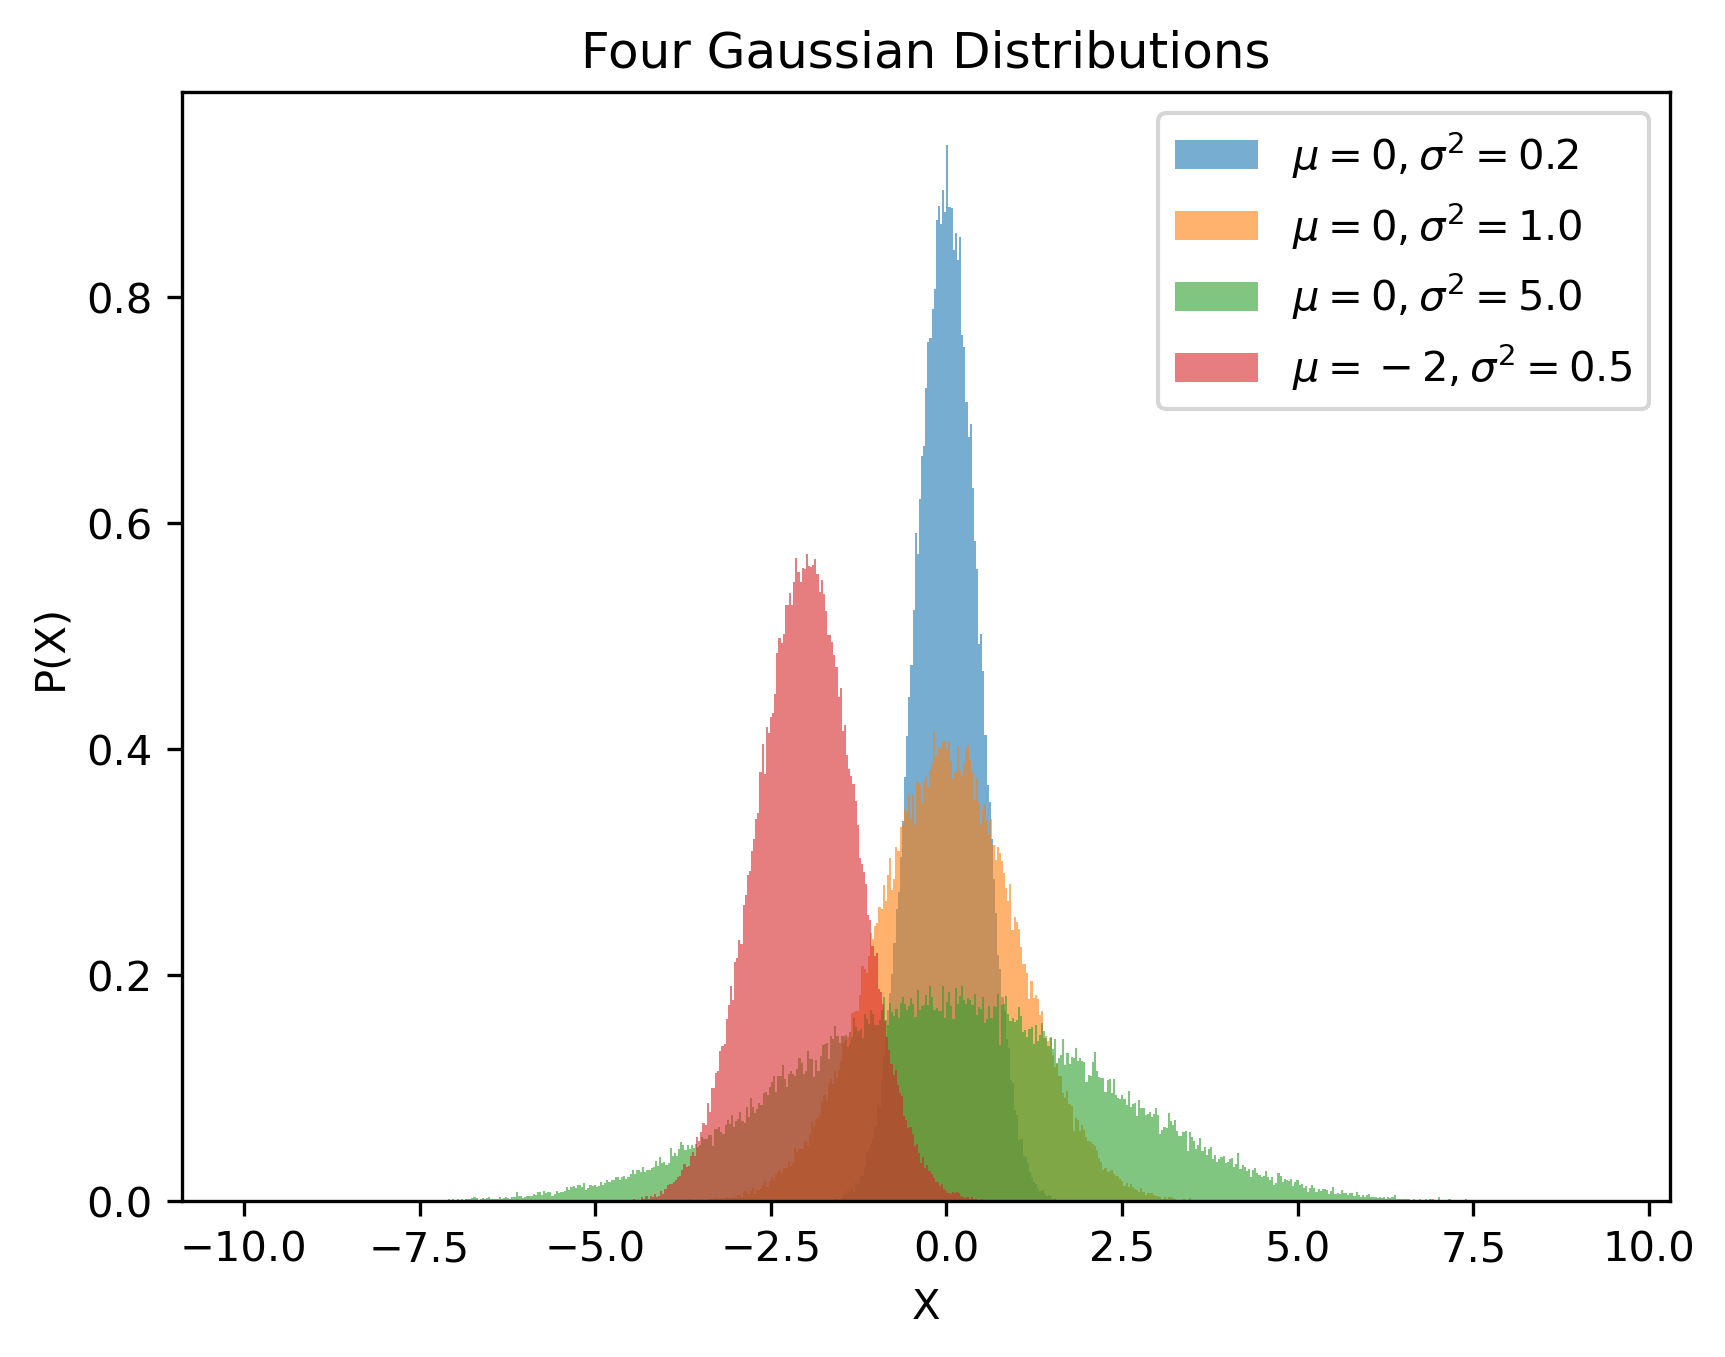
\includegraphics[width=0.6\textwidth]{img/2c.png}
	\caption{Histograms of Gaussian distributions generated using algorithm $\cal{A}$}
\end{figure}

\subsection*{Task D}
\begin{lstlisting}[language=Python, caption={Python code to implement Galton board and plot their histograms for $h=10,50,100$}, label=lst:galton]
import matplotlib as mpl
import matplotlib.pyplot as plt
import numpy as np

mpl.rcParams["figure.dpi"] = 300

N = 10**5
hs = [10, 50, 100]
for i, h in enumerate(hs):
    pockets = []
    for _ in range(N):
        dirs = np.random.randint(2, size=h) # uniformly sample h values from {0, 1}
        x = np.sum(dirs * 2 - 1) # map 0 to -1 and 1 to 1, and sum them to get final pocket
        pockets.append(x)
    plt.hist(pockets, bins=100, density=True)
    plt.xlabel("pocket")
    plt.ylabel("normalized count")
    plt.title(f"Galton board with h={h}")
    plt.savefig(f"2d{i + 1}.png", bbox_inches="tight")
    plt.show()
\end{lstlisting}
\begin{figure}[H]
	\centering
	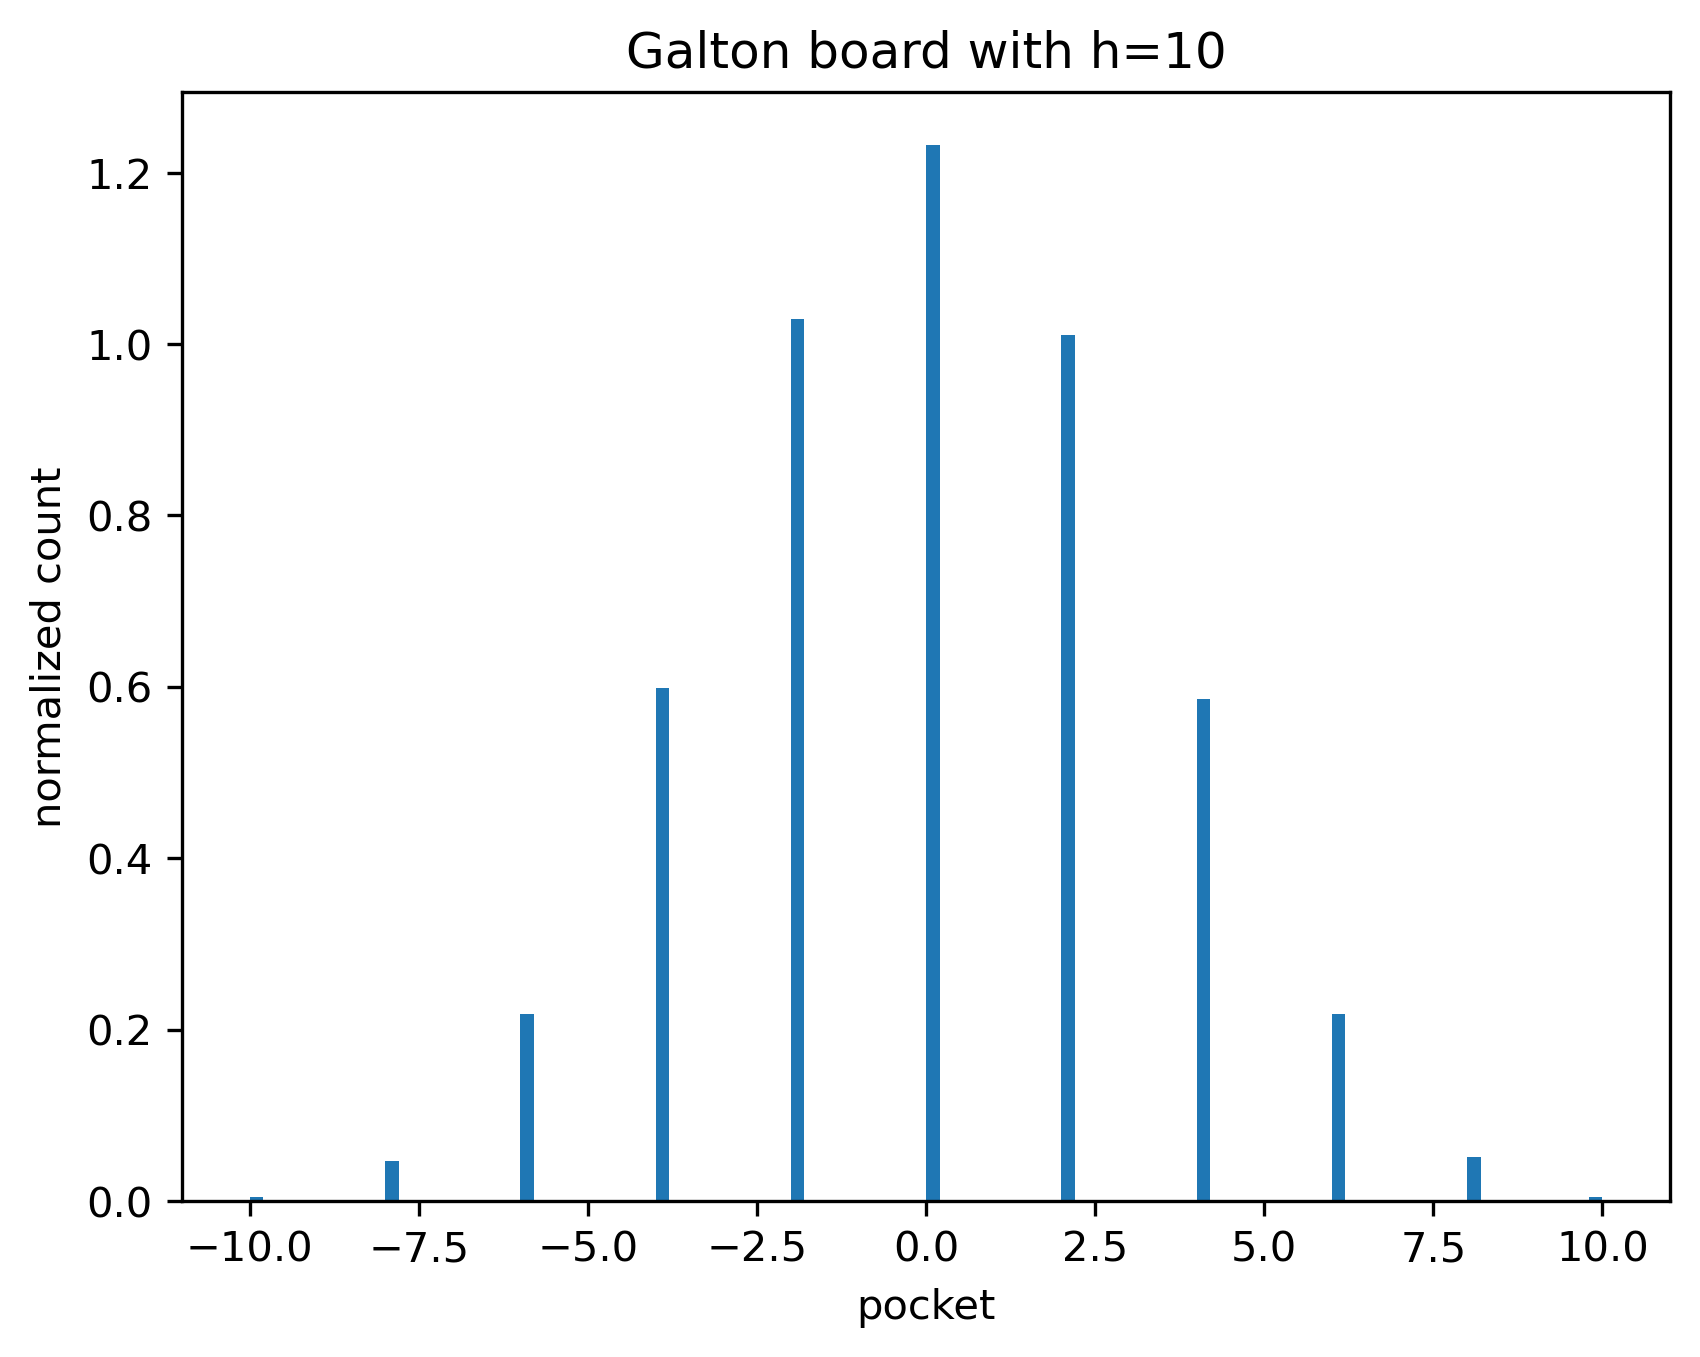
\includegraphics[width=0.6\textwidth]{img/2d1.png}
	\caption{Galton board with $h=10$}
\end{figure}
\begin{figure}[H]
	\centering
	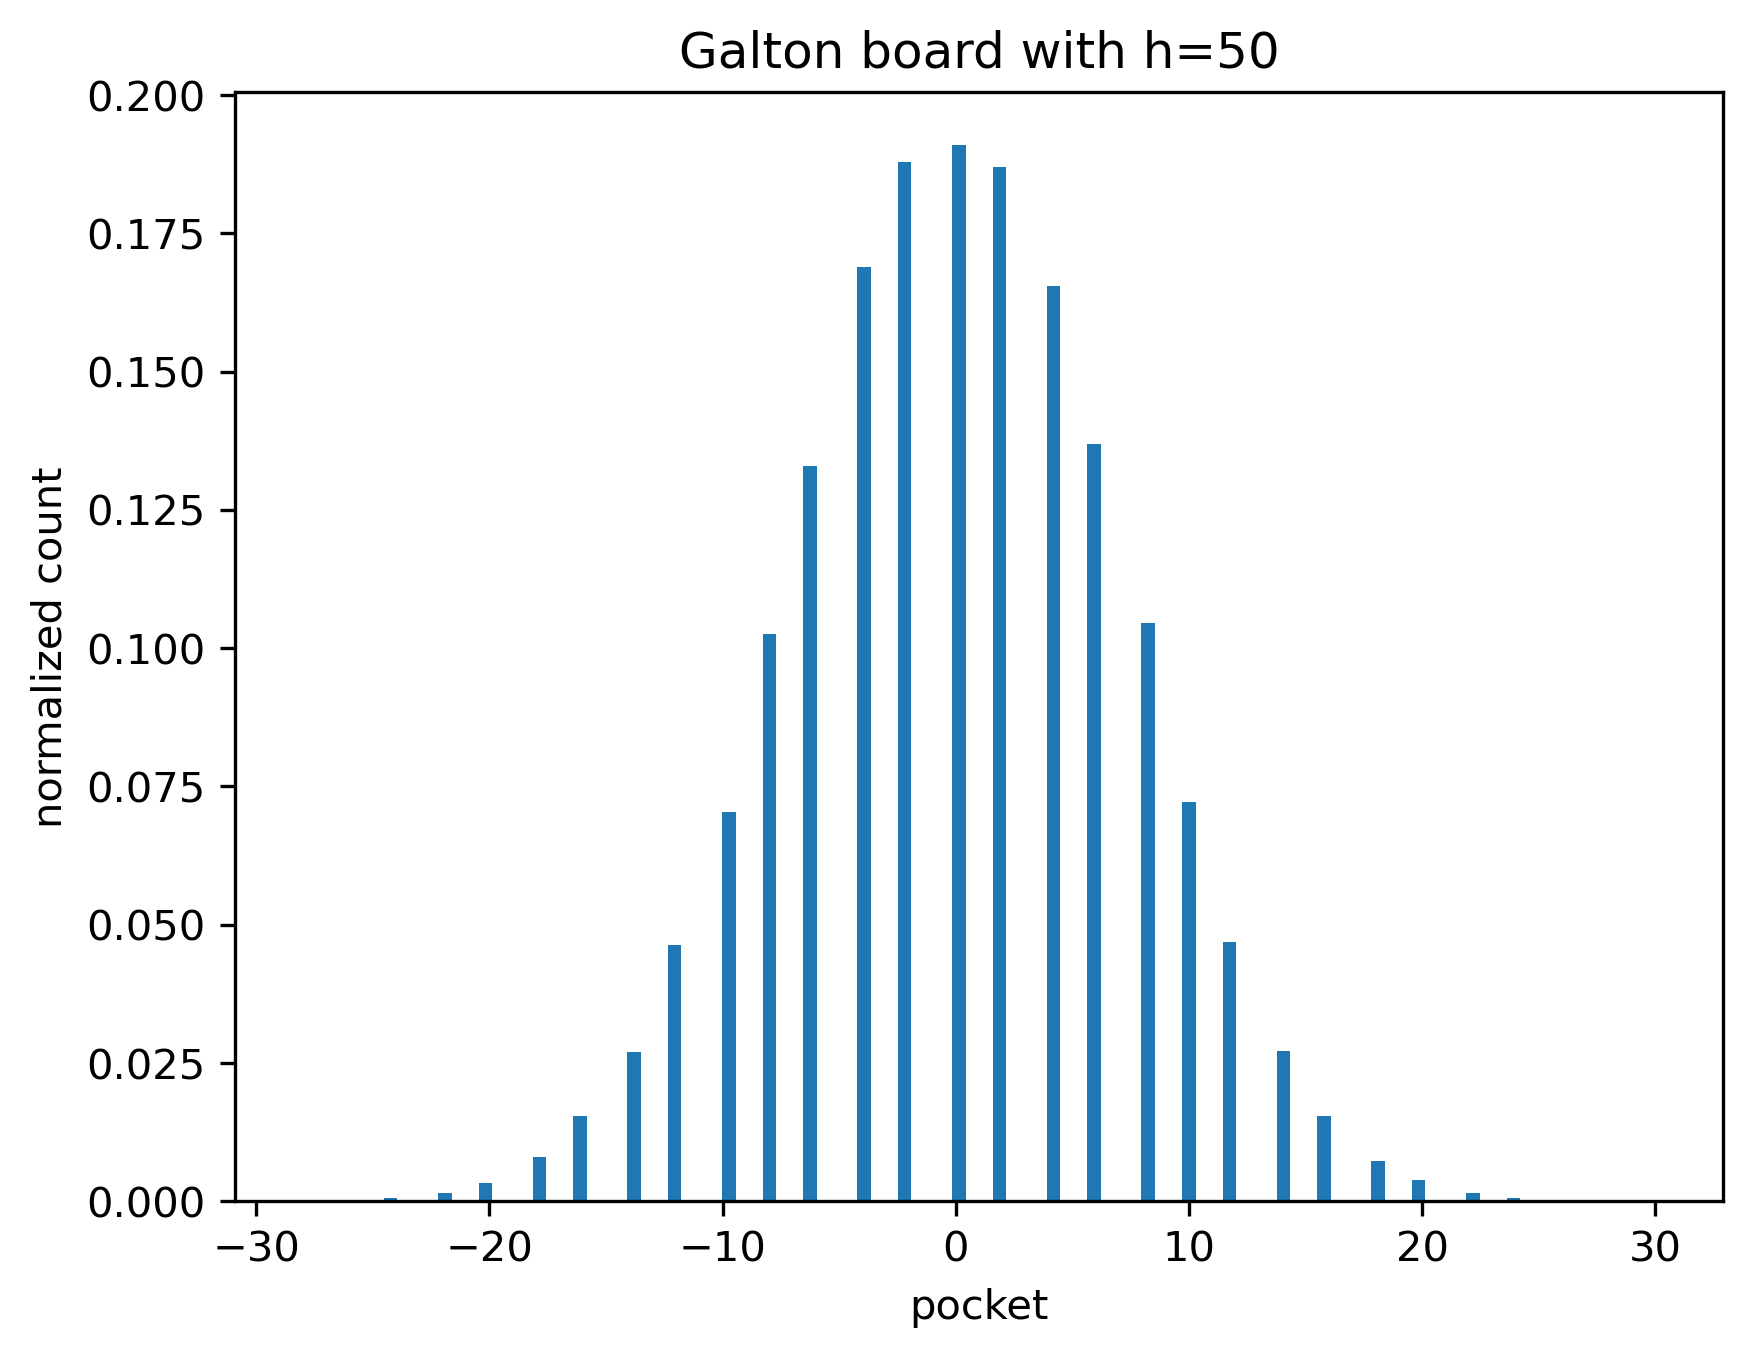
\includegraphics[width=0.6\textwidth]{img/2d2.png}
	\caption{Galton board with $h=50$}
\end{figure}
\begin{figure}[H]
	\centering
	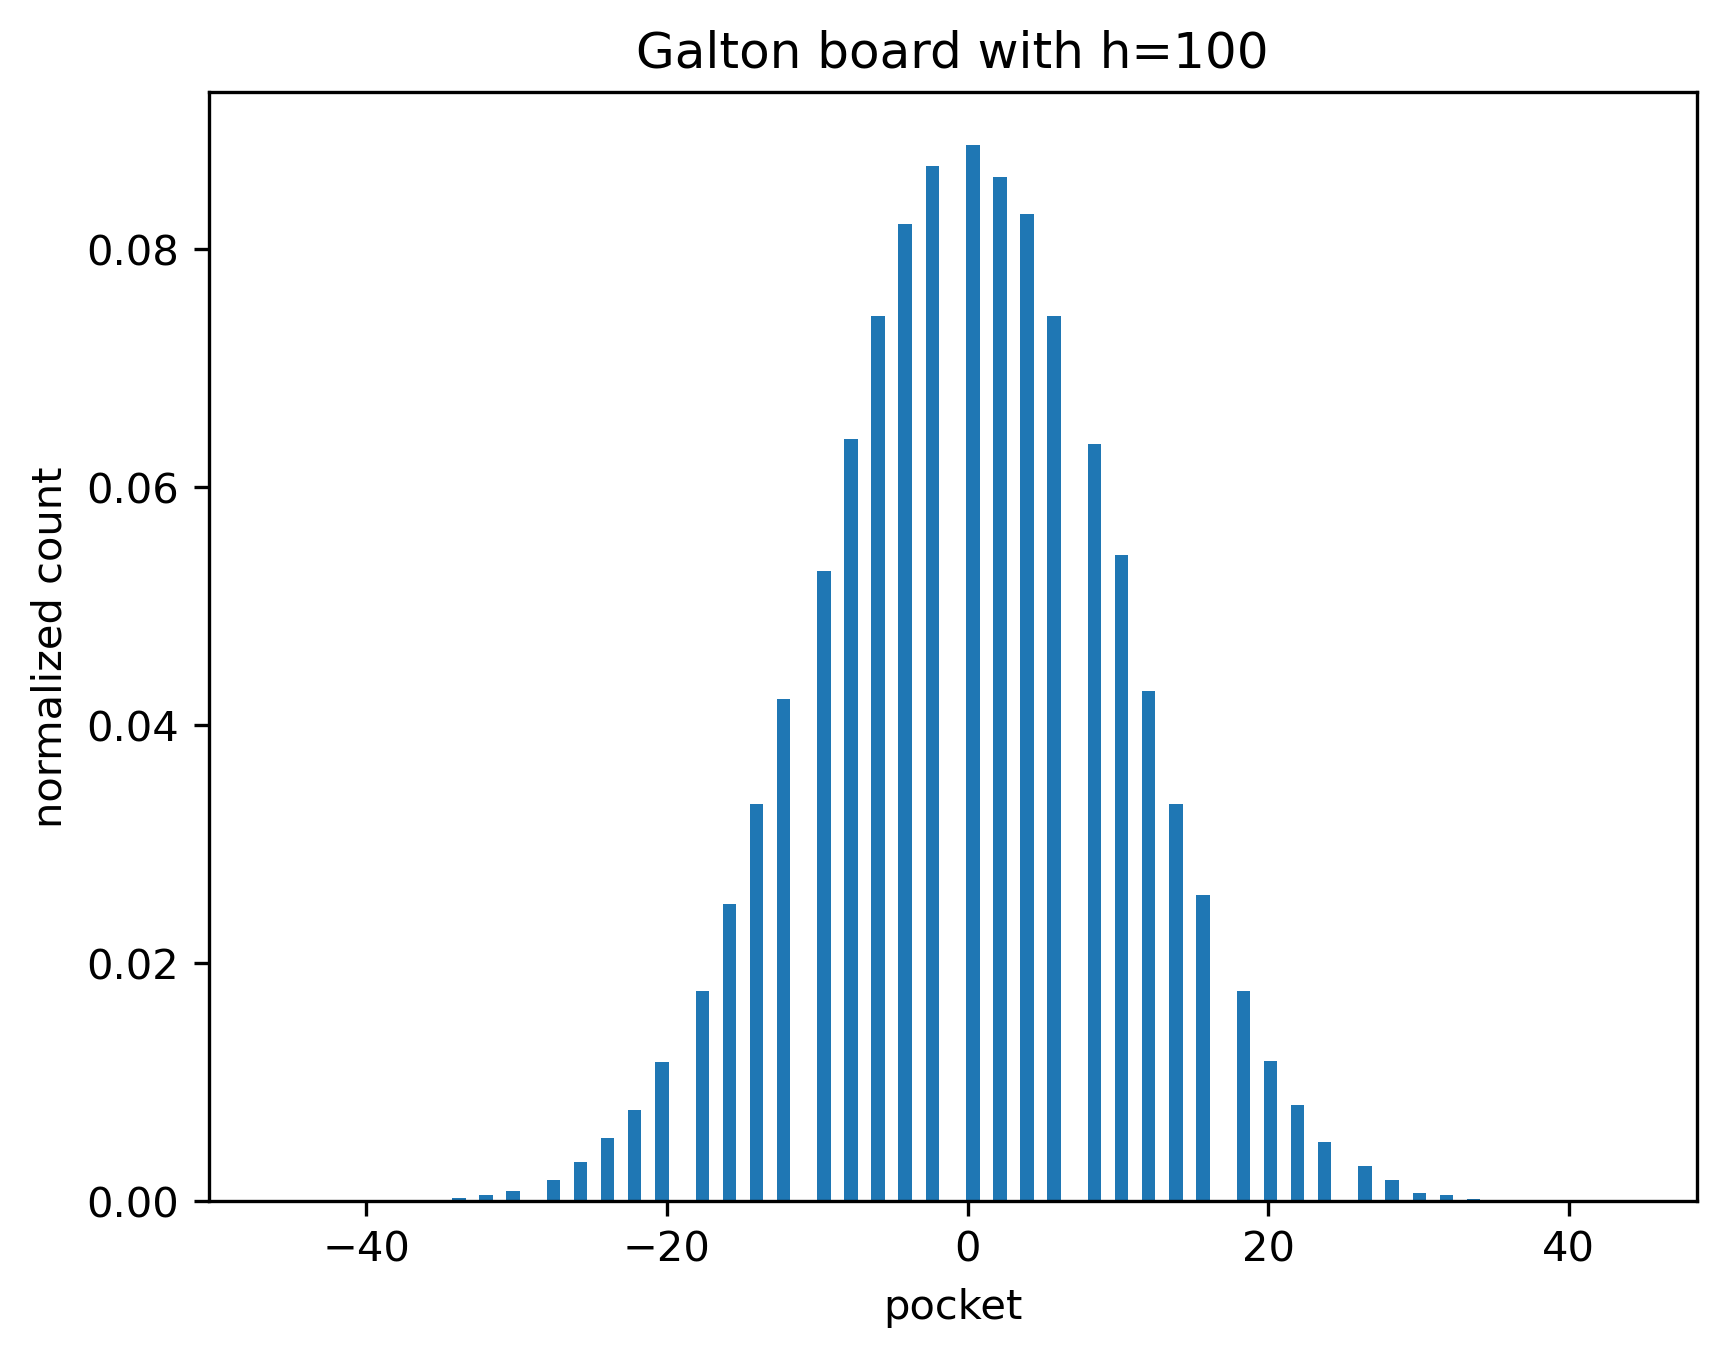
\includegraphics[width=0.6\textwidth]{img/2d3.png}
	\caption{Galton board with $h=100$}
\end{figure}

\subsection*{Task E}
We are given a Galton Board of depth $h$, and random variable $X\in \left\{-h,-h+2,\cdots,0,2,\cdots,h-2,h\right\}$ to describe the pocket in which a ball lands.

\subsubsection*{Computing $P_h[X=2i]$ \normalfont for $i\in\{-k,-k+1,\cdots,k-1,k\}$}
Consider random variable $Y \in \{-1,1\}$, which represents the direction of the ball after hitting a peg, $-1$ for left and $1$ for right.
We have random variables $Y_j$ for $j\in\left\{1,2,\cdots,h\right\}$ representing the directions of the ball after hitting each peg.
Note that $X = \sum_{j=1}^{h}Y_j$.\\

\begin{claim}
	For $X=2i$ and $i \in \left\{-k,-k+1,\cdots, -1,0,1,\cdots,k-1,k\right\}$, we need to have $k - i$ left movements.
\end{claim}
\begin{proof}
	Consider $a$ number of left movements, and $h-a=2k-a$ number of right movements.
	We need to find a solution to the following equation.
	\begin{align*}
		-1 \cdot a + 1 \cdot (2k-a) & = 2i    \\
		2k - 2a                     & = 2i    \\
		\therefore    a             & = k - i
	\end{align*}
	This gives us the number of left movements. Note that $a$ is always non-negative.
\end{proof}

Once we have the number of left movements, we can choose any $k-i$ pegs out of $h$ pegs to be the left movements.
And at each peg, the probability of going left or right is equal to $1/2$.
So, we can write the probability of $X=2i$ as:
\begin{align}
	\therefore P_h[X=2i] = \binom{h}{k-i} \left(\frac{1}{2}\right)^h \label{eq:probx2i}
\end{align}

\subsubsection*{Showing that $P_h$ converges to a Gaussian Distribution}
\begin{remark}
	A couple of well-known approximations that we will use in our proof are:
	\begin{align}
		(1+x)^n & \approx 1 + nx \label{eq:binomial-approx}                                   \\
		e^{-x}  & \approx 1 - x \label{eq:exp-approx}                                         \\
		n!      & \approx \sqrt{2\pi n} \left(\frac{n}{e}\right)^n \label{eq:stirling-approx}
	\end{align}
	\cref{eq:binomial-approx} is valid for $x$ small and $n$ large.
	\cref{eq:exp-approx} is valid for $x$ small.
	\cref{eq:stirling-approx} is valid for large $n$.
\end{remark}
We first substitute $2i$ for $i$, and $k$ for $\dfrac{h}{2}$ in \cref{eq:probx2i}.
\begin{align*}
	P_h[X=i] & = \binom{h}{\frac{h-i}{2}} \left(\frac{1}{2}\right)^h
\end{align*}
Now, we will simplify the binomial coefficient term using \cref{eq:stirling-approx}.
\begin{align*}
	\binom{h}{\frac{h-i}{2}}\left(\frac{1}{2}\right)^h & = \frac{h!}{2^h\left(\frac{h-i}{2}\right)!\left(\frac{h+i}{2}\right)!}                                                                                                                                         \\
	                                                   & \approx \frac{\sqrt{2\pi h}\left(\frac{h}{e}\right)^h}{2^h\sqrt{2\pi \frac{h-i}{2}}\left(\frac{h-i}{2e}\right)^\frac{h-i}{2}\sqrt{2\pi \frac{h+i}{2}}\left(\frac{h+i}{2e}\right)^\frac{h+i}{2}}                \\
	                                                   & = \sqrt{\frac{2\pi h}{\pi(h-i)\pi(h+i)} }\left(\frac{h}{2e}\right)^h \left(\frac{\frac{h-i}{2e}}{\frac{h+i}{2e}}\right)^\frac{i}{2}\left(\frac{1}{\frac{h-i}{2e} \frac{h+i}{2e}}\right)^\frac{h}{2}            \\
	                                                   & = \sqrt{\frac{2 h}{\pi \left(h^2-i^2\right)}}\left(\frac{h}{2e}\right)^h \left(\frac{1-\frac{i}{h}}{1+\frac{i}{h}}\right)^\frac{i}{2}\left(\frac{(2e)^2}{h^2-i^2}\right)^\frac{h}{2}                           \\
	                                                   & = \sqrt{\frac{2 h}{\pi \left(h^2-i^2\right)}}\left(\frac{h}{2e}\right)^h \left(\frac{1-\frac{i}{h}}{1+\frac{i}{h}}\right)^\frac{i}{2}\left(\frac{(2e)^2}{h^2\left(1-\frac{i^2}{h^2}\right)}\right)^\frac{h}{2} \\
	                                                   & = \sqrt{\frac{2 h}{\pi \left(h^2-i^2\right)}}\left(\frac{h}{2e}\right)^h \left(\frac{1-\frac{i}{h}}{1+\frac{i}{h}}\right)^\frac{i}{2}\left(\frac{2e}{h}\right)^h\left(1-\frac{i^2}{h^2}\right)^{-\frac{h}{2}}  \\
	                                                   & = \sqrt{\frac{2 h}{\pi \left(h^2-i^2\right)}} \left(\frac{1-\frac{i}{h}}{1+\frac{i}{h}}\right)^\frac{i}{2}\left(1-\frac{i^2}{h^2}\right)^{-\frac{h}{2}}
\end{align*}
Since we are given that $i << \sqrt{h}$, we can approximate $h^2-i^2 \approx h^2$. Also, we can use \cref{eq:binomial-approx} and \cref{eq:exp-approx} to make the following approximations:
\begin{align*}
	\left(1-\frac{i}{h}\right)^\frac{i}{2}        & \approx 1-\frac{i^2}{2h}  \approx e^{-\frac{i^2}{2h}}  \\
	\left(1+\frac{i}{h}\right)^{-\frac{i}{2}}     & \approx 1 - \frac{i^2}{2h} \approx e^{-\frac{i^2}{2h}} \\
	\left(1-\frac{i^2}{h^2}\right)^{-\frac{h}{2}} & \approx 1 + \frac{i^2}{2h} \approx e^\frac{i^2}{2h}
\end{align*}
Now, we simply the expression with the new approximations.
\begin{align*}
	\binom{h}{\frac{h-i}{2}}\left(\frac{1}{2}\right)^h & \approx \sqrt{\frac{2 h}{\pi h^2}}e^{-\frac{i^2}{2h}}e^{-\frac{i^2}{2h}}e^{\frac{i^2}{2h}} \\
	                                                   & = \sqrt{\frac{2}{\pi h}} e^{-\frac{i^2}{2h}}                                               \\
	\therefore P_h[X=i]                                & \approx \frac{1}{\sqrt{\pi k}} e^{-\frac{i^2}{4k}}
\end{align*}
This shows that the distribution of $X$ converges to a Gaussian distribution as $h$ increases.

